
%% ****** Start of file apstemplate.tex ****** %
%%
%%
%%   This file is part of the APS files in the REVTeX 4.2 distribution.
%%   Version 4.2a of REVTeX, January, 2015
%%
%%
%%   Copyright (c) 2015 The American Physical Society.
%%
%%   See the REVTeX 4 README file for restrictions and more information.
%%
%
% This is a template for producing manuscripts for use with REVTEX 4.2
% Copy this file to another name and then work on that file.
% That way, you always have this original template file to use.
%
% Group addresses by affiliation; use superscriptaddress for long
% author lists, or if there are many overlapping affiliations.
% For Phys. Rev. appearance, change preprint to twocolumn.
% Choose pra, prb, prc, prd, pre, prl, prstab, prstper, or rmp for journal
%  Add 'draft' option to mark overfull boxes with black boxes
%  Add 'showkeys' option to make keywords appear
%\documentclass[aps,prb,twocolumn,superscriptaddress]{revtex4-1}
\documentclass[aps,prl,preprint,superscriptaddress]{revtex4-2}
%\documentclass[aps,prl,reprint,groupedaddress]{revtex4-2}

% You should use BibTeX and apsrev.bst for references
% Choosing a journal automatically selects the correct APS
% BibTeX style file (bst file), so only uncomment the line
% below if necessary.
%\bibliographystyle{apsrev4-2}
\usepackage{graphicx}
\usepackage{amsmath,amsthm,amssymb,mathtools}
\usepackage{amsfonts}
\usepackage{bm}
\usepackage{color}
\frenchspacing
%\graphicspath{/pics/}
%\graphicspath{{~/data/KannanLu/exp623/article/}}
\usepackage{listings}
\usepackage{color}
\definecolor{codegreen}{rgb}{0,0.6,0}
\definecolor{codegray}{rgb}{0.5,0.5,0.5}
\definecolor{codepurple}{rgb}{0.58,0,0.82}
\definecolor{backcolour}{rgb}{0.95,0.95,0.92}
% \definecolor{backcolour}{rgb}{0.18,0.18,0.18}
\lstdefinestyle{mystyle}{
    backgroundcolor=\color{backcolour},
    commentstyle=\color{codegreen},
    keywordstyle=\color{magenta},
    numberstyle=\tiny\color{codegray},
    stringstyle=\color{codepurple},
    basicstyle=\footnotesize,
    breakatwhitespace=false,
    breaklines=true,
    captionpos=b,
    keepspaces=true,
    numbers=left,
    numbersep=5pt,
    showspaces=false,
    showstringspaces=false,
    showtabs=false,
    tabsize=2
}
\lstset{style=mystyle}

\begin{document}

% Use the \preprint command to place your local institutional report
% number in the upper righthand corner of the title page in preprint mode.
% Multiple \preprint commands are allowed.
% Use the 'preprintnumbers' class option to override journal defaults
% to display numbers if necessary
%\preprint{}

%Title of paper
\title{Independent Component Analysis}

% repeat the \author .. \affiliation  etc. as needed
% \email, \thanks, \homepage, \altaffiliation all apply to the current
% author. Explanatory text should go in the []'s, actual e-mail
% address or url should go in the {}'s for \email and \homepage.
% Please use the appropriate macro foreach each type of information

% \affiliation command applies to all authors since the last
% \affiliation command. The \affiliation command should follow the
% other information
% \affiliation can be followed by \email, \homepage, \thanks as well.

%\email[]{Your e-mail address}
%\homepage[]{Your web page}
\author{Kittithat Krongchon}
\author{Kannan Lu}
\affiliation{Department of Physics, University of Illinois at Urbana-Champaign, Urbana, IL 61801, USA}

%Collaboration name if desired (requires use of superscriptaddress
%option in \documentclass). \noaffiliation is required (may also be
%used with the \author command).
%\collaboration can be followed by \email, \homepage, \thanks as well.
%\collaboration{}
%\noaffiliation

\date{\today}

\begin{abstract}
Indenpendent component analysis (ICA) is an unsupervised learning technique that is widely used in extracting independent factors in image, sound and medical signals. In this document, we review the basic notions of the ICA including mathematical formulations and detailed algorithms. We also implement different algorithms based on higher-order statistics and information theoretic approaches. These algorithms are applied to sound signal disentanglement and EEG blinking signal removal with success.     
\end{abstract}

\maketitle

\section{Introduction}
Independent component analysis (ICA) is one of the classical unsupervised learning techniques that is used to seperate out latent variables or reduce dimensions. The motivation of the development of this technique is based on very commom problems. For instance, in reality, source signals are often corrupted with 'noise'. Or in other words, data are composed by mutiple independent source signals. To isolate the signals from different sources, ICA can be a good choice. The famous example is the 'cocktail party problem', where the sound detectors record the superposition of various sound signals from different sources in the party. The goal is to seperate out the observed signal into sounds from each different source. Since we do not know what the sources are and how these signals are mixed, this type of problem is called 'blind source separation' (BSS). ICA is widely used in images, sounds, stock market and medical signals. ICA can also be viewed as an extension of principle component analysis (PCA), where the latter maximizes the second order statistics (covariance matrix of data). ICA maximizes higher-order statistics or simply tries to look for independent components not just uncorrelated components. In Fig.~\ref{fig:ICA_vs_PCA}, we show the ICA components $IC_{i}$ and PCA components $PC_{i}$ learned from the observed data $x_{i}$ with the original sources $s_{i}$ sampled from uniform distribution independently. Clearly. the ICA learned the independent components correctly but the PCA did not in this case. 

In this paper, we will review mathematical background of the ICA technique, the detailed algorithm implementation and several realizations in typical examples. 

\begin{figure}[b]
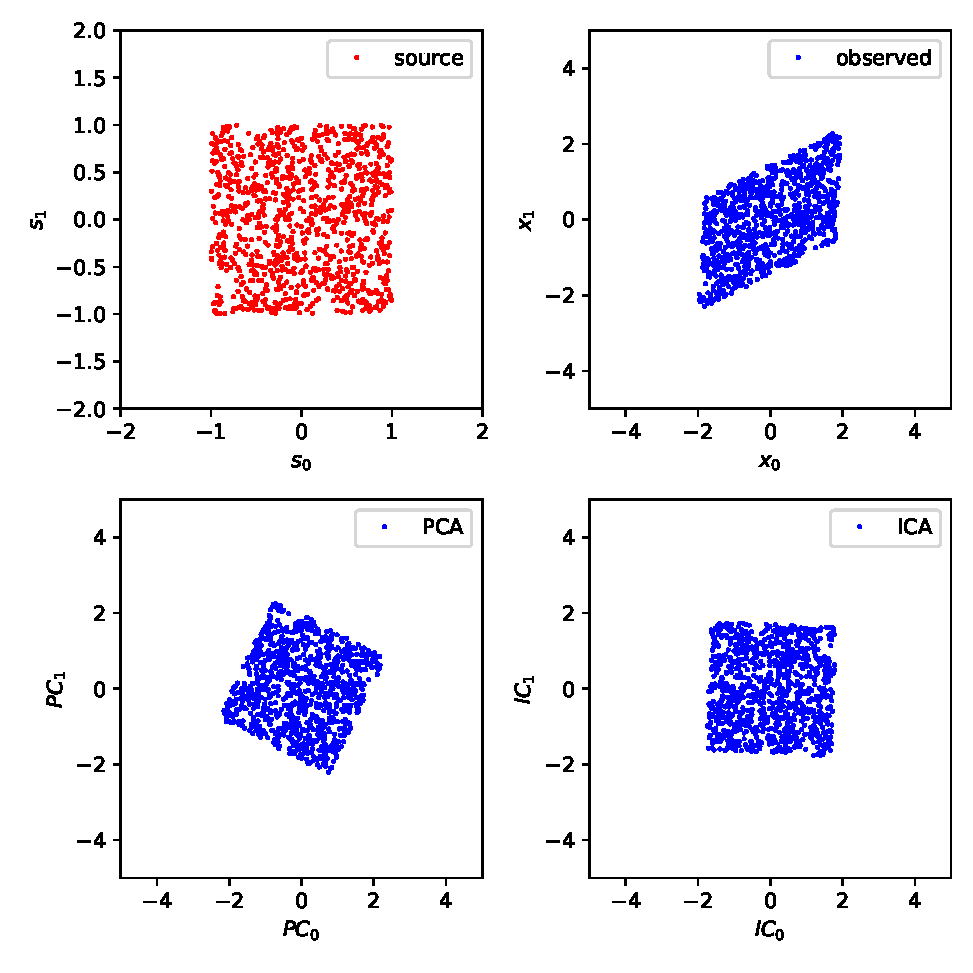
\includegraphics[width=0.8\textwidth]{scripts/ICA_vs_PCA.pdf}
 \caption{\label{fig:ICA_vs_PCA} shows the PCA and ICA result of unmixing the observed data $x_{i}$ generated from two independent uniform variables $s_{i}$. The algorithm is based on maximizing the higher order moments. }
\end{figure}
% Put \label in argument of \section for cross-refe(WHAT DOES THIS LAST SENTENCE MEAN?)rencing
%\section{\label{}}
%\subsection{}
%\subsubsection{}

\section{Mathematical Background}
\subsection{Definition of the problem and notations}
Before we delve into the detailed mathematical formalisms, we first define the notations that we will use throughout the whole document. We will use boldface capital letters $\bf{A}$ for matrices, boldface lowercase letters $\bf{a}$ for vectors and ordinary lower case letters $a$ for scalars. We will use subscripts for denoting the components of matrices (i.e. $A_{ij})$ and vectors (i.e. $a_{i}$). Notice that these letters are not in boldface as they mean the specific component, which is just a scalar in $ \rm I\!R$. Superscripts are reserved for indexing different samples. For instance, $m$ samples of vector $\bf{a}$ can be denoted as $\bf{a}$$^{(k)}$ where $k = 1, 2, ..., m$. Following these conventions, we denote the original signal to be $\bf{s}$$^{(i)} \in \rm I\!R^{d}$. We consider the standard setting where the $d$ dimensional signals $\bf{s}$$^{(i)} \in \rm I\!R^{d}$ ($d$ original sources) are mixed and observed by $d$ detectors $\bf{x}$$^{(i)} \in \rm I\!R^{d}$ (i.e. the cocktail party scenario). That is there is a linear map between the $\bf{s}$$^{(i)}$ and $\bf{x}$$^{(i)}$, $\bf{x}$$^{(i)}$ $=$ $\bf{A}$$\bf{s}$$^{(i)}$, where $\bf{A} \in \rm I\!R^{d\times d}$ is known as the mixing matrix. The whole idea of ICA is to learn the inverse of the mixing matrix $\bf{W} = \bf{A}$$^{-1}$ from the observed data $\bf{x}$$^{(i)}$, known as the un-mixing process. The learned independent components are denoted by $\bf{u} = \bf{W}\bf{x}$. This can be done in several different ways based on ideas of seperating non-Gaussian signals, and the original signals being independent. We will in this section discuss various mathematical formulations. All these various theoretical frameworks are based on several constraints of the problem. These are:\\
(1) The number of sensors is larger than number of sources. This ensures that the mixing matrix is full rank; \\
(2) The sources at each sample (time) are mutually independent; \\
(3) At most one source is normally distributed. \\
Without these conditions, the BSS problem is ill-defined. For simplicity, we will also restrict the discussion to cases where the number of detectors and sources are the same. However, a generalization to condition (1) is feasible and the algorithms discussed in the following sections will still work.

Based on these definitions, we need to talk about some ambiguities embedded in the symmetry of the problem and justify that if the origianl signals are all Gaussians, they cannot be learned through the un-mixing. There are two ambiguities that usually do not affect the practical application, namely the permutation ambiguity and the scaling ambiguity. It is trivial to see that the ordering of the original sources \{$s_{j}$\} is ambiguous. In the case of scaling, if the original signal $\bf{s}$ is scaled by a non-zero constant to be $c\bf{s}$ where $c \neq 0$. Then the mixing matrix $\bf{A}$ can be scaled by $1/c$ and resulting in the same observed data $\bf{x}$$ = \frac{1}{c}\bf{A}$$c\bf{s}$. This scaling ambiguity can be furtherly extended with regard to each component of the original signal. That is, for a particular component $j$, if we scale the component by $c_{j}$ the corrsponding column of the mixing matrix can be scaled by $1/c_{j}$ to have the observed data unchanged (i.e. $x_{i} = \sum_{j}\frac{1}{c_{j}}A_{ij}c_{j}s_{j}$).  


The other ambiguity that matters for the practical application is that the original sources cannot all be distributed as Gaussians. Or to be more precise, in order to seperate the independent components, we require that the original signals can only have at most one component to be sampled from a Gaussian distribution, i.e. $s_{j}$ $\sim \mathcal{N}(\mu,\,\sigma^{2})$ for at most one $j$. Let's consider the case when all the original independent signals are Gaussians. That is, $s_{j}$ $\sim \mathcal{N}(\mu_{j},\,\sigma_{j}^{2})$ for $j = 1, 2, ..., d$. Then given the mixing matrix $\bf{A}$, we have 
\begin{equation}
\mathbb{E}_{\bf{s}}[\bf{x}] = \bf{A}\mathbb{E}[\bf{s}] = \bf{A}\bm{\mu}
\end{equation}
and 
\begin{equation}
Cov[\bf{x}] = \mathbb{E}_{\bf{s}}[\bf{As}\bf{s}^t\bf{A}^{t}]-\mathbb{E}_{\bf{s}}[\bf{As}]\mathbb{E}[(\bf{As})^{t}] =  \bf{A}\bm{\Sigma}\bf{A}^{t}-\bf{A}\bf{M}\bf{A}^{t}
\end{equation} 
, where $\bf{M}$ and $\bm{\Sigma}$ are diagonal matrices of $\rm I\!R^{d\times d}$ with diagonal elements to be \{$\mu_{j}^{2}$\} and \{$\sigma_{j}^{2}$\}, respectively. Due to the scale ambiguity, this is the same as considering normally distributed signals with unity variance. Since each column $j$ of the mixing matrix $\bf{A}$ can be scaled by $\sigma_{j}$, $\tilde{\bf{A}}_{:j} = \sigma_{j}\bf{A}_{:j}$ and correspondingly the signal needs to be scaled by $1/\sigma_{j}$, $\tilde{s_{j}} = \frac{s_{j}-\mu_{j}}{\sigma_{j}}$. Then, 
\begin{equation}
Cov[\bf{x}] = \tilde{\bf{A}}\bf{I}_{d\times d}\tilde{\bf{A}}^{t}.
\end{equation}
Now, if we consider a rotation $\bf{R} $$\in O(d)$ acting on the scaled source signals $\bf{\tilde{s}}$. The mixing matrix then changes to $\tilde{\bf{A}}\bf{R}$. Unpon this rotation, we would observe $\bf{x'}$ as $\bf{x'} = \tilde{\bf{A}}\bf{R}\tilde{\bf{s}}$. $\bf{x'}$ is again normally distributed and has covariance matrix,
\begin{equation}
Cov[\bf{x'}] = \tilde{\bf{A}}\bf{R}\bf{I}_{d\times d}\bf{R}^{t}\tilde{\bf{A}}^{t} = \tilde{\bf{A}}\bf{I}_{d\times d}\tilde{\bf{A}}^{t}. 
\end{equation} This simply means that whether the sources are rotated or not the observed data will be distributed as $\mathcal{N}(0, \tilde{\bf{A}}\tilde{\bf{A}}^{t})$. Thus, because of the rotational symmetry of the multivariate Gaussian distribution, we cannot seperate and obtain the original source signals. These derivations also indicate that given the observed data $\bf{x}$, we can whiten the data and it will not affect the seperated signals (up to scalings and mean translations).   

\subsection{Higher order statistics approach}

The non-Gaussianity thus directly provide us with the methodologies used in finding the independent component. Notice that the PCA only finds the uncorrelated components but not necessarily independent. The ICA tries to find independent components where the joint distibutions can be factorized into marginal distributions by investigating into higher-order moments. There are multiple moment-based objective functions have been used along the development of ICA. We will define some of the notations and stick to one of the moment-based objective functions in this paper.  

As we discussed previously, we have the freedom to whiten the observed signals and we will denote the whitened observed data as $\tilde{\bf{x}}$, where each component is $\tilde{x_{j}} = \frac{x_{j}-\mathbb{E}[x_{j}]}{\sigma_{x,j}}$. The skewness, kurtosis and excess kutosis are defined as $$ \gamma(x) := \mathbb{E}[\tilde{x}^{3}], \beta(x) := \mathbb{E}[\tilde{x}^{4}], \kappa(x) := \beta(x)-3 $$.
The objective function is a convex combination of the squared third and fourth cumulants defined as follows,
\begin{equation}
L_{\alpha}(\bf{w}) := \alpha \gamma^{2}(\bf{w}^{t}\tilde{\bf{x}}) + (1-\alpha)\kappa^{2}(\bf{w}^{t}\tilde{\bf{x}})
\end{equation},
where $\alpha \in [0, 1]$ and $\bf{w}^{t}\bf{w}$$ = 1$.

%1) Optimizing Kurtosis (high-order based moment approach) (Mick)
%2) non-gaussianity  (Mick)
%3) Maximum likelihood estimation (Kannan)
%    - Minimizing mutual information (min KL divergence)

\subsection{Information theoretic approach}

Apart from the moment based approaches, there are several information theoetic formalisms. Here in this section, we will review all different information theoretic frameworks and show that essentially they are equivalent. Then we will talk about the learning rules for these theoretical formulations in the subsequant setion. 

The centralized quantity in all these formalisms is the mutual information, which is defined as the KL divergence of the multivariate distribution of the observed data $\bf{x}$ and product of all its marginal distributions, i.e. 
\begin{equation}
I(\bf{x}) = \sum_{\bf{x}}p(\bf{x})\log\frac{p(\bf{x})}{\prod_{i}p_{i}(x_{i})}.
\end{equation} $I(\bf{x})$ is non-negative and is 0 if and only if the $\bf{x}$ are independent. Several different information theoretic approaches have been formulated in history and can be unified in the concept of minimizing the mutual information of the seperated components $\bf{u} = \bf{W}\bf{x}$. 

One of them is a key finding in neural networks, that is, maximizing information between inputs $\bf{x}$ and outputs $\bf{y}$ implies that the output distributions are factorized, thus minimizes the mutual information in the outputs $\bf{y}$. Maximizing the information between inputs and outputs is to maximize the output joint entropy $H(\bf{y}) = \sum_{i}H(y_{i}) - I(\bf{y})$, where $I(\bf{y}) = \sum_{\bf{y}}p(\bf{y})\log\frac{p(\bf{y})}{\prod_{i}p_{i}(y_{i})}$ is the mutual information in the outputs $\bf{y}$. The mutual information is non-negative and is zero if and only if $\bf{y}$ are marginalized. Recall that in neural network, the output is given by the nonlinearity $y_{i} = g_{i}(\bf{w}_{i}^{t}\bf{x})$ $:= g_{i}(u_{i})$, thus $p(y_{i}) = \frac{p(u_{i})}{|\frac{\partial g_{i}}{\partial u_{i}}|}$. The maximum is therefore obtained by considering the gradient,
\begin{equation}
\frac{\partial H(\bf{y})}{\partial \bf{W}} = \frac{\partial (-I(\bf{y}))}{\partial \bf{W}} -\frac{\partial}{\partial \bf{W}}\sum_{i} \mathbb{E}[\log \frac{p(u_{i})}{|\frac{\partial g_{i}}{\partial u_{i}}|} ]. 
\end{equation}
This implies that the nonlinear function $g_{i}$ in the neural network $y_{i} = g(\bf{w}_{i}^{t}\bf{x})$ is a cdf of the source distribution $s_{i}$ in order to kill the second term. Together with the constraint that the outputs are marginalized, this gradient is zero. Therefore, a good estimation of the cdf of the source signal improves drastically the performance of ICA. Notice that, if $I(\bf{y}) = 0$, the $\bf{u} = \bf{W}\bf{x}$ should also satisfy $I(\bf{u}) = 0$ as $g_{i}$ is an invertible monotonic function. Hence, the neural network approach can be eventually reduced to minimizing the mutual information $I(\bf{u})$.

Another way to formulate this is to maximize the negentropy $J(u_{i})$, which is the KL divergence $D(p(u_{i})||p_{G}(u_{i}))$ between $p(u_{i})$ and Gaussian distribution $p_{G}(u_{i})$ with the same mean and covariance as $p(u_{i})$. Recall that the Gaussian distribution has maximum entropy constrained with the mean and covariance. The negentropy thus measures non-Gaussianity. Requiring that the $\bf{u}$ can be factorized and decorrelated, the sum of negentropies can be written as 
\begin{align}
\sum_{i}J(u_{i}) &= \sum_{i}D(p(u_{i})||p_{G}(u_{i})) \\
&= \sum_{i}p(u_{i})\log\frac{p(u_{i})}{p_{G}(u_{i})} \\
&= \sum_{\bf{u}}p(\bf{u}) \log\frac{\prod_{i}p(u_{i})}{\prod_{i}p_{G}(u_{i})} \\
&= \sum_{\bf{u}}p(\bf{u}) \log\frac{\prod_{i}p(u_{i})}{p_{G}(\bf{u}_{i})} \\
&= \sum_{\bf{u}}p(\bf{u}) \log\frac{\prod_{i}p(u_{i})}{p(\bf{u})} + \sum_{\bf{u}}p(\bf{u})\log\frac{p(\bf{u})}{p_{G}(\bf{u})} \\
&= D(\prod_{i}p(u_{i})||p(\bf{u})) + J(\bf{u}) \\
&= -I(\bf{u}) + J(\bf{u}) \\
& = -I(\bf{u}) - H(\bf{u}) - \sum_{\bf{u}}p(\bf{u})\log p_{G}(\bf{u}) \\
& = -I(\bf{u}) - H(\bf{x}) - \log(|det(\bf{W})|) - \frac{1}{2}\log((2\pi e)^{d}det(<\bf{u}, \bf{u}^{t}>))\\
&= -I(\bf{u}) - H(\bf{x}) - \frac{1}{2}\log((2\pi e)^{d}).
\end{align} In the derivation, the $\bf{u}$ are uncorrelated so the covariance matrix is identity. Therefore, maximizing the negentropy is equivalent to minimizing mutual information in $\bf{u} = \bf{W}\bf{x}$. 

Lastly, for the maximum likelihood estimation approach, we want to maximize the log likelihood over all samples observed upon choosing a parametrized distribution $\hat{p}_{s}(\bf{w}_{i}\bf{x})$ satisfying $p(\bf{x}) = \prod_{i}^{d}\hat{p}_{s}(\bf{w}_{i}\bf{x})|\bf{W}|$. The log-likelihood is 
\begin{equation}
l(\bf{W}) = \frac{1}{N}\sum_{j=1}^{N}(\sum_{i=1}^{d}\log(\hat{p}_{s}(\bf{w}_{i}\bf{x}^{(j)}))+\log|\bf{W}|).
\end{equation}   
If the approximation $\hat{p}_{s}(\bf{w}_{i}\bf{x})$ are close to the actual pdf, the first term is approximately $-\sum_{i}H(\bf{w}_{i}\bf{x})$ and is equal to the negative of the mutual information up to an additive constant of the total entropy of $\bf{x}$. Hence, all these historical information theoretic approaches are equivalent and the key idea is to approximate the probability distribution of the sources correctly. Historically, there has been several proposed parametric distributions for approximating super-Gaussian or sub-Gaussian distributions. We will proceed to discuss the algorithm associated with the information based approach in the next section. 

\section{Algorithms}
In this section, we will discuss some of the common algorithms based on the previous mathematical formalisms. We will categorize them into moment-based approaches and information-based approaches. In either case, the problem is equivalent to an optimization problem. There are some detailed differences on how this optimization problem is implemented, i.e. ordinary gradient descent, Newton's method or fixed point algorithm. We will simply specify what we implemented for various examples that we will discuss later. 
\subsection{Moment-based approach}
In this method, we maximize the non-Gaussianity given by
\begin{align}
J(Y) \propto \{E[G(Y)] - E[G(V)]\}^2,
\end{align}
where $Y$ is a random variable of zero mean and unit variance, which can be achieved by whitening the data, and $V$ is a Gaussian variable also of zero mean and unit variance. In function forms of $G_1$ and $G_2$ should not grow too fast to be robust. The following choice of $G$ is proposed by Hyvärinen and Oja~\cite{hyvarinen2000independent}.
\begin{align}
G_1(u) &= \frac{1}{a_1} \log (\cosh a_1 u). \\
G_1^{\prime}(u) &= \tanh(a_1 u).
\end{align}
We want to find the extrema of $E[G(Y)]$ to maximize $J(Y)$ under the constraints
\begin{align}
E[(w^T x)^2] = \| w\|^2 = 1.
\end{align}
From the Kuhn--Tucker conditions, the extremum condition is satisfied when
\begin{align}
E[x g(w^Tx)] - \beta w &= 0.
\end{align}
This equation can be solved by using Newton's method.
Let $F(w)$ denote the left-hand side of the equation, which we are trying to solve.
We update the value of $w$ in each iteration according to the following equation.
\begin{align}
w_{n+1} &= w_n - \frac{F(w_n)}{F^{\prime}(w_n)} \\
&= w_n - \frac{E[x g (w_n^T x)] - \beta w_n}{E[g^{\prime}(w_n^T x)] - \beta} \\
&= \frac{w_n E[g^{\prime}(w_n^T x)] - \beta w_n - E[x g (w_n^T x)] + \beta w_n}{E[g^{\prime}(w_n^T x)] - \beta} \\
&= \frac{w_n E[g^{\prime}(w_n^T x)] - E[x g (w_n^T x)]}{E[g^{\prime}(w_n^T x)] - \beta}.
\end{align}
\subsection{Information theoretic approach}
Based on what has been discussed in the previous section, we can approximate the source signal distribution with a parametrized pdf. There are multiple choices here tailored to different problems. A default choice is to assume the cdf of the source signal can be approximated by a sigmoid function $g(s_{i}) = \frac{1}{1+e^{-s_{s}}}$, thus the pdf is $p(s_{i}) = g'(s_{i})$. Notice that this pdf is super-Gaussian. This means that ICA based on this pdf works well when the distribution of original sources have heavy tails and sharp peak around center. Recall the log-likelihood (without normalization), 
\begin{align}
l(\bf{W}) &= \sum_{j=1}^{N}(\sum_{i=1}^{d}\log(\hat{p}_{s}(\bf{w}_{i}\bf{x}^{(j)}))+\log|\bf{W}|) \\
&= \sum_{j=1}^{N}(\sum_{i=1}^{d}\log(g'(\bf{w}_{i}\bf{x}^{(j)}))+\log|\bf{W}|)
\end{align}    
\section{Applications}
We implement FastICA according to the formalism described in the previous section.
The algorithm is applied to a following set of signal functions.
\begin{align}
s_1 &= \sin(2 t). \\
s_2 &= \mathrm{sign} [\sin(3 t)]. \\
s_3 &= \frac{1}{2\pi} (t~\mathrm{mod}~2\pi).
\end{align}
The mixing matrix is taken to be
\begin{align}
A &= \begin{bmatrix}
1 & 1 & 1 \\
0.5 & 2 & 1 \\
1.5 & 1 & 2
\end{bmatrix}.
\end{align}
The result from our implementation and FastICA are shown in Fig.~\ref{fig:sklearn}.
% \begin{figure}
% \includegraphics{scripts/sklearn.pdf}
% \caption{\label{fig:sklearn} FastICA results using our code and \lstinline{sklearn.decomposition.FastICA}}
% \end{figure}


%3) example: sound single decomposition
%4) EEG % (https://towardsdatascience.com/independent-component-analysis-ica-a3eba0ccec35)
%5) stock price


\section{How to check the robustness and convergence}
% Amari metric, ref "ELements of Statistical Learning", p.570

%1) check if the performance matrix is identity (Te-won Lee, p. 51)
\begin{align}
W A &= I.
\end{align}

%2) check how fast w changes (ICA_projectionPursuit1612.05445.pdf, p. 12)


\section{what if two of the sources are dependent}
%s3 = signal.sawtooth(2*np.pi*time) # saw tooth signal
%s4 = s1 + s2
%s5 = s1 - s2

\section{Discussions and Conclusions}
1) review the traditional development from 1990s
2) recent advances and development from 2000s  
3) what happens when there are multiple Gaussian components

\bibliography{paper}{}

\end{document}
\grid
\grid
\grid
